% \documentclass{twocolumn,jsarticle}

\documentclass[twocolumn,10pt]{jarticle}

\setlength{\headheight}{0mm}
\setlength{\headsep}{0mm}
\setlength{\columnsep}{2zw} 

\usepackage[dvipdfmx]{graphicx}

\pagestyle{empty}


\title{交通システムとIoT}
\author{増井俊之 \\ 慶應義塾大学 環境情報学部}
\date{2019年3月29日}
\begin{document}
\maketitle

\thispagestyle{empty}

\abstract{
  電車やバスや自動車などの交通システムは
  長年にわたって現代社会に不可欠なインフラとなっている。
  また、パソコンやスマホのようなコンピュータや様々なセンサが
  ネットに接続されたIoT環境も社会のインフラとなりつつあるが、
  両インフラを統合的に活用するシステムはまだまだ発展途上である。
  交通システムとIoTを融合したシステムやサービスの可能性について考察する。
}

\section{はじめに}
  
ここ何年か「IoT」という単語がバズワードになっていたが、
最近はこの単語を聞く機会が減ってきた気がする。
あらゆる場所のセンサがインターネットに接続されることによって
世の中が激しく便利になることが期待されたのだろうが、
革新的な応用が充分開発されていないのかもしれない。

情報処理学会の学会誌「情報処理\footnote{
  \textsf{https://www.ipsj.or.jp/magazine/magazine.html}
}」では2019年初頭にIoT特集が組まれている。
2019年2月号の「社会を変えるIoT」という特集では
近年のIoT応用例が多数紹介されていたが、
水産業のために海の状況をモニタするシステム、
ノリ養殖支援システム、
養豚支援システムのような第一次産業での利用が最も多く、
その次に多いものが介護支援や子ども見守りシステムのような
弱者支援システムであった。
また、2019年3月号は「水産業におけるIoT」という特集で、
水産クラウド、
スマート水産データベース、
定置網での魚種判別、
赤潮監視システム
などが紹介されていた。

無線接続された沢山のセンサとコンピュータを実世界に配置して活用する技術は
従来は「センサネットワーク」と呼ばれることが多かった。
前述のような一次産業的な応用において
センサネットワーク技術が重要であることは間違いないが、
センサネットワークをベースとした新しいサービスは
あまり出現していないようである。
せっかくセンサやコンピュータが身の回りに沢山存在するのだから、
人間と一緒にセンサやコンピュータが移動したり、
人間とコンピュータのインタラクションも利用できできたり、
人間自体がセンサの一部になったり、
もっと面白い\textbf{アクティブなIoT}システムが
広まってほしいものである。

アクティブなIoTとは以下のような特徴をもつものである。

\begin{itemize}
  \setlength{\itemsep}{0cm} % 項目間  
  \item 人間とセンサを区別しない
  \item センサやコンピュータも人間も移動する
  \item 人間のアクションや状態がセンサ情報になる
  \item センサと人間がインタラクションを行なう
  % \item 人間間のコミュニケーションに利用する
  % \item 動き回る人間がセンサとして働く
  \item 人間がアクチュエータとして行動することもある
\end{itemize}

\section{交通系IoT}
  
電車やバスなどの公共交通機関は
大規模なアクティブなIoTを構築しやすい環境だといえる。
自動車や自転車もアクティブなIoTの構成要素として期待できる。
%
交通サービスで運用される「交通系IoT」は以下のような
特徴を利用できる。

\begin{itemize}
  \setlength{\itemsep}{0cm} % 項目間  
  \item 数が膨大
  \item 大規模に移動する
  \item センサと駅や車輛やが紐づいている
  \item センサとユーザが紐づいている
  \item 普通の人間活動に紐づいている
\end{itemize}

  % \item 電車とは限らない
% \item 自転車サーバ

電車は膨大な数の人間やセンサの運搬システムであるにもかかわらず、
そのことはほとんど活用されていない。
また、沢山の人が利用する駅施設や店でも
IoT活用はまだまだである。

交通系IoTには巨大な可能性があるはずだが、
キラーアプリケーションがまだみつかっていないのだろう。

% センサを持った人間が歩きまわる
% 人間がアクティブに何かをタッチする
% 人間をセンサにする話
% HASC
% 
% 情報の共有 /コミュニケーションへの利用
% 
% 自分情報の記録
% どこに行ったか
% 日記になる

\section{交通系IoT活用事例}

自動改札の導入で磁気切符が主流になったり
交通系RFIDカードが導入されたりといった変化は
記憶に新しいところであり、、
トイレやエスカレータやエキナカなどは昔に比べると激しく改善されてきているが、
基本的な駅や電車の使い方は100年以上あまり変わっていないようにも見える。
交通系IoTによりこれがどう変わるかを考えてみる。

\paragraph{混雑の回避}

次のバスや電車がいつ来るのか? どれぐらい混んでいるのか?
といった情報はとても重要であるにもかかわらず、
2019年になっても充分な情報がユーザに伝わっていない。
%
車輛内のセンサやGPSを利用すれば
現在位置や混雑状況は簡単に計測できるし、
それをネット上に公開することも簡単なのにもかかわらず、
こういうサービスが提供されていないのは不思議なことである。
%
「電車やバスとはこういうものだから多少の不便は仕方がない」と
思いこんでいる人が多いため、
IoT技術が実生活の改善に反映されていないのだと思われる。

物理学者/エッセイストとして知られる寺田寅彦は、
1922年(大正11年)に「電車の混雑について」という随筆\footnote{
  \small{\textsf{https://www.aozora.gr.jp{\slash}cards{\slash}000042{\slash}files{\slash}2449\_11267.html}}
}で、すいた電車に乗るためのコツを述べている。

\begin{quotation}
``必ずすいた電車に乗るために採るべき方法はきわめて平凡で簡単である。
  それはすいた電車の来るまで、気長く待つという方法である。''
\end{quotation}

\begin{figure}[htbp]
  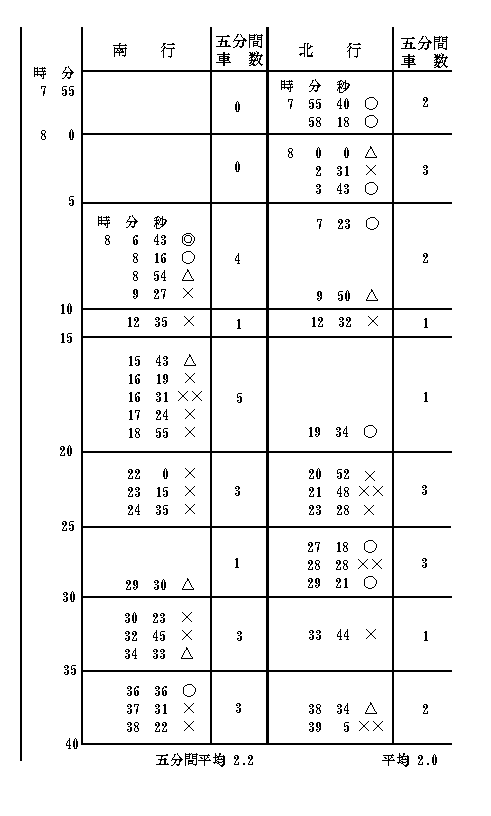
\includegraphics[clip,width=7.0cm]{./terada.png}
  \caption{寺田寅彦による電車の観察結果}
\end{figure}

しばらく待った後に来る電車は混雑しているものであり、
客が一斉にそれに乗ろうとするとその電車はさらに混むはずなので、
混んだ電車はやり過ごして次の電車を待つのが得策だということらしい。
これは100年前の東京の市電の話であり、
時刻表通りに正確に運行される電車では状況は異なるかもしれないが、
現代でもバスの状況は似たようなものであろう。

寺田寅彦の時代とは異なり、
現在は様々なIoT技術を利用できるのだから、
電車やバスの混雑具合や運行状況の情報は苦労なく取得して共有できるはずなのに、
100年前と同じような悩みが解消されていないのは驚くべきことかもしれない。

\paragraph{席を確保する}
  
席が空いていない場合でも、現在座っている人が降りる駅がわかれば、
その人の前で席が空くのを待つことができる。
「靴を見ればだいたいどの駅で降りるかわかる」と豪語する人\footnote{
  \textsf{https://www.facebook.com/knnkanda}
}の話を聞いて驚いたことがあるが、
そういう特殊能力が無くても
センサ技術を利用すれば降りる駅を判定できる可能性がある。

お茶の水女子大学の笹川真奈氏\footnote{
  \textsf{https://scrapbox.io/mitou-meikan/笹川\_真奈}
}は、
2014年の
未踏IT人材発掘・育成事業\footnote{
  \textsf{https://www.ipa.go.jp/jinzai/mitou/portal\_index.html}
}で「電車で効率よく座るための支援アプリケーションの提案と実装」というシステムを開発した。
このシステムでは、
乗客が持っているスマホなどのBluetooth信号を計測してデータベース記録することにより、
スマホを持つ人がどの駅で乗ったり降りたりするかを予測して降りそうな人を
捜すようになっている。
このようなデータベースを構築するのは大変だし、
プライバシの懸念など様々な問題はあるが、
センサやネット情報を駆使することにより
電車で快適に過ごす可能性があることを示した点は面白い。

\paragraph{乗り換え情報など}
  
どの電車に乗れば早く目的地につくのか、どう歩けばうまく乗り換えられるのか、
といった情報は重要であるが、このような情報を得ることは現在でも簡単ではない。
乗換案内\footnote{
  \textsf{https://www.jorudan.co.jp/norikae/}
}のようなサービスを使えばこういった情報を知ることができるが、
電車の運行状況や混雑状況も考慮して電車を選べるアプリはまだ
広く利用されていない。

スマホの乗換案内アプリなどで検索を行なった場合、
スマホは自分の行きたい場所を知っているわけだから、
電車の運行状況や混雑状況、駅の構造などをもとにして
「右の階段を昇って4番線に移動」のように 最適な行動を
提案することも可能なはずであるが、
そういう情報は普通は提供されていないので
案内表示などを見て考えて行動する必要がある。
駅のサイネージに遅延などの運行状況を表示する努力は進んでいるが、
乗客がそれを注意して見て理解して最適な行動を考えなければならないようでは
まだまだだであろう。

電車に間に合うための行動を支援する
駅.Locky\footnote{
  \textsf{http://eki.locky.jp/site/top}
}というアプリケーションがある。
普通の時刻表を利用する場合、
ある電車に乗れるかどうかを調べるためには
現在時刻、時刻表、自分の位置を考えて
かなり頭を使わなければならないが、
駅.Lockyでは、
現在時刻や時刻表について調べなくても
「次の電車まで何分あるか」という情報だけを簡単に見ることができるので、
ユーザの負担が軽くなる。
電車に間に合うか調べるためには時刻表を見なければならないと
筆者も思い込んでいましたが、
そもそもから発想した全く異なる解法を提示しているところには感心した。

\paragraph{情報の提示/通知}

ドアの上の液晶ディスプレイなどで電車の状況を知らせてくれる車両が
増えいるが、 情報提示の手法や内容はまだまだ工夫の余地があるし、
案内ディスプレイの数はまだ少ない。
このような車内ディスプレイは
路線名や行先を表示していることが多いが、
ほとんどの人は路線や行先を確認してから電車に乗っているはずですから
そういう情報を車内に常に表示しておくことは重要ではないと思われます。
それよりも、現在どこを走っているのか/現在どの駅に停まっているのか/次に停まる駅はどこか、
といったアクティブに変化する情報を主に表示するべきであろう。
有用な情報が提示されたとき、その情報を記憶するのは面倒である。
ディスプレイに提示された情報や中吊り広告などの情報を手に入れたいと思ったとき、
内容をスマホなどにすぐコピーできてもよいのだが、
そういうことができるサービスは存在しない。
提示場所と時刻がわかれば提示情報の内容は簡単にわかるので、
提示場所を示すIDをスマホで読み取るか入力するだけで情報取得できるはずである。

ユーザの現在位置をもとにして電車のIDがわかり、
車両番号がわかれば現在乗ってる車両に関する情報を正確に得ることができる。
車両情報を利用した情報提示サービスはもっと出てきてほしい。
次の駅のトイレの空き具合がわかるサービスが欲しい。

\paragraph{情報共有システム}
  
周囲の人間と匿名で情報交換したいと思うことが時々ある。
結婚式の写真や観光写真などを隣の人と交換したいような場合、
メールアドレスやSNSのIDを教えずに情報だけを交換したいような場合です。
こういう場合のため、一時的な「合言葉」(e.g. 123456)のようなものを決めて情報交換する
サービスがあれば便利である。
電車の場合、車両IDなどを利用して匿名コミュニケーションを行なうことが
できるだろう。
同じ車両の乗客の間で「冷房キツすぎるない?」とか「事故の影響どうなってるの?」
といったコミュニケーションができると便利だろう。

一方、自分が乗っている車両のIDをFacebookなどで公開すれば、
家族や友達に現在の状況を伝えることができます。
友達が隣の車両に乗っていても気付くことは難しいですが、こ
ういった情報を使えば新しいコミュニケーションが可能になるだろう。

\paragraph{車内や駅のエンターテインメント}
  
辛い満員電車でも、楽しい音楽や動画を楽しんでいれば苦痛はやわらぐものである。
最近の飛行機は尾翼などに装着されたカメラの映像を座席で楽しむことができるが、
電車の運転席から見える風景を席で見ることができれば面白いだろう。
旅先の電車で、土地の名物や観光名所や歴史を聞くことができれば楽しいだろう。
%
通勤路でも、途中駅のイベントやレストランなどのおすすめ情報がわかれば
立ち寄ってみる気になるかもしれない。
駅のサイネージなどにちょっとしたゲームエンターテインメントを用意しておき、
待ち時間を楽しくしたりコミュニケーションに活用したりできる可能性もある。
ちょっとした工夫により、様々なエンターテインメントを提供できる可能性がある。


\section{増井研の取り組み}

増井研究室では、
このようなアクティブなIoTを可能にする各種のシステムを
開発している。

\begin{itemize}
  \setlength{\itemsep}{0cm} % 項目間  
  \item Linda \\
    単純で柔軟な分散通信ネットワーク
  \item BabaScript \\
    ユーザがIoT要素となるプログラミング言語
  \item Gear \\
    満員電車のような苛酷な環境でも
    コンテンツ閲覧可能なインタフェース
  \item Golddfish \\
    スマホを「実世界GUI」端末にする
  \item ConnecTouch \\
    Suicaによるコミュニケーション支援
\end{itemize}

    
%   \item タッチ場所
%   \item 吊り革
%   \item ポスタ

また、今後はプライバシ処理や
新しい行動認証手法なども研究開発していきたいと考えている。

将来はアクティブな交通系IoTが普及していくことは間違いない。
誰もが簡単にそういう環境で生活できるような
「イディオム」のデザインも考えていきたい。


% \section{交通系IoTの課題}
% 
% 
% 実世界IoTのイディオム / 使い勝手
% プライバシ
% みんなTカードは使うから大丈夫か?
% 
% 提案
% 認証
% Suica + EpisoPass
% 行動履歴認証
% 
% 人生100歳時代のIoT


\end{document}
